\documentclass[10pt]{article}

\addtolength{\oddsidemargin}{-.875in}
\addtolength{\evensidemargin}{-.875in}
\addtolength{\textwidth}{1.75in}

\addtolength{\topmargin}{-.875in}
\addtolength{\textheight}{1.75in}

\openup 1em

%macro for commenting
\usepackage{color}
\newcommand{\leo}[1]{{\color{blue}{\it leo: #1}}}

% \newcommand{\Xbeta}{ X_i \theta}
\newcommand{\xbeta}{ x_i \beta}
\newcommand{\xtheta}{ x_i \theta}
% \newcommand{\xbetaij}{ x_{ij}^T \theta}
\newcommand{\sgamma}{s_{ij}^T\gamma_i}

\usepackage[round]{natbib}

\usepackage{rotating}
\usepackage{graphicx}
\usepackage{subcaption}

\usepackage{float}


\usepackage{amsthm,amsmath} 
\usepackage{amssymb}
\usepackage{subcaption}
\usepackage{nicefrac}

\newtheorem{theorem}{Theorem}
\newtheorem{lemma}{Lemma}
\newtheorem{corollary}{Corollary}
\newtheorem{remark}{Remark}


\usepackage{algorithm}
\usepackage{algpseudocode}

%\usepackage{mhequ}
\newcommand{\be}{\begin{equation}\begin{aligned}}
\newcommand{\ee}{\end{aligned}\end{equation}}
\newcommand{\bb}[1]{\mathbb{#1}}
\newcommand{\mc}[1]{\mathcal{#1}}
\DeclareMathOperator{\Binom}{Binomial}
\DeclareMathOperator{\No}{No}
\DeclareMathOperator{\PG}{PG}
\DeclareMathOperator{\IG}{Inverse-Gamma}
\DeclareMathOperator{\Ga}{Gamma}
\DeclareMathOperator{\Bern}{Bernoulli}
\DeclareMathOperator{\U}{Uniform}
\DeclareMathOperator{\Poi}{Poisson}
\DeclareMathOperator{\NB}{NB}
\DeclareMathOperator{\cov}{cov}
\DeclareMathOperator{\var}{var}
\DeclareMathOperator{\diag}{diag}
\DeclareMathOperator{\Diag}{Diag}
\newcommand{\KL}[2]{\textnormal{KL}\left(#1 \parallel #2\right)}

\DeclareMathOperator{\bigO}{\mc O}



\thispagestyle{empty}
\baselineskip=28pt

\title{\textbf{Fast Bayesian Tensor Factorization\\ with Empirically Estimated Factors}}
\author{Leo Duan}
\date{}
\begin{document}

\maketitle

I am proposing a computationally efficient Bayesian tensor factorization. This is a special Tucker decomposition with factors fixed on empirically estimated/chosen values. The empirical estimates can be viewed as quick approximation to the ``ideal'' basis associated to a core tensor of lowest rank, highest sparsity or very simple structure (e.g. diagonal). With the imperfection, the core would be less parsimonious, but still remain sparse and low rank.

Although a constraint is applied on the factors, the flexibility of the tensor model is unscathed, when the factors contain the basis of the original tensor. Taking advantage of the sparsity in the core, a multi-way Dirichlet shrinkage prior is assigned to the scales of the core parameters, effectively reducing the core to small size.

To facilitate parallel computing and good posterior mixing, I choose empirical factors residing on Stiefel manifold. This induces conditional independence on the core parameters and allow efficient block sampling.

This method has a potential wide range of applications. For example, one could pre-assign Fourier basis as an empirical factor for high-dimension multivariate spatial tensor, and treat the core tensor as a non-parameteric estimate of spectrum. In this report, I focus on a dimension reduction application over a group of large binary adjacency matrices. I fix the empirical factor to be the bases from singular value decomposition (SVD) applied on the mean graph, inducing a low-rank and near-diagonal plane in the 3-way core.

\section{Motivating Application: Dimension Reduction of a Group of Large Adjacency Matrices}

Consider a three-way binary tensor $A\in \{0,1\}^{n\times n \times m}$. This tensor is a compilation of $m$ subjects' connectome graphs, and each graph is a symmetric $n\times n$ binary matrix describing the connectivity among the $n$ vertices. Let $A_{i,jk}$ denote the connectivity between vertices $j$ and $k$ in the $i$th adjacency matrix $A_{i}$.

The motivating application is to obtain a collection of low dimensional representation of the adjacency matrix for each subject, preserving most of the across-subject difference. For one matrix, SVD is routinely used to produce a diagonal vector, which is commonly low rank. For multiple matrices, it is natural to consider its extension to a {\it joint diagonalization}.

\be
\label{parafac_over_i}
A_{i,jk} \sim \Bern(\Phi( \psi_{i,jk})),\\
\psi_{i,jk}=\sum_{r=1}^{\kappa} d_{i,r} u_{j,r} u_{k,r},\\
\Psi_{i}= \{ u_{j}^T  D_{i} u_{k}\}_{j,k} = U^T D_iU
\ee
for $i=1,\ldots,m, \quad  j=2,\ldots n, \quad k=1,\ldots,(j-1)$ and $\psi_{i,jk}=\psi_{i,kj}$; $\Phi(.)$ is the standard normal cumulative probability, $u_{(.)}$ and $d_{(.)}$ are scalars; $\kappa$ is the rank of of this decomposition; $D_{i}=\diag\{d_{i,1},\ldots d_{i,\kappa}\}$, $u_j = \{ u_{j,1},\ldots, u_{j,\kappa}\}'$ is a vector and $U=[ u_1 || \ldots || u_n ]$ is the corresponding $ \kappa \times n$ matrix. Since the diagonal element $A_{i,jj}$ is not defined on the graph, we treat $\psi_{i,jj}=\sum_{r=1}^{\kappa} d_{i,r} u_{j,r} u_{j,r}$ as a latent variable.

The set of diagonal vectors in $\{D_i\}_{i=1,\ldots, m}$ can then be used to represent the full adjacency matrices. This model is in fact a reparameterization of a parallel factor analysis (PARAFAC) decomposition. Letting  $d_{i,r} = \lambda_r  d^*_{i,r}$, a rank-$\kappa$ PARAFAC can be obtained:

\be
\psi_{i,jk}=\sum_{r=1}^{\kappa} \lambda_r  d^*_{i,r} u_{j,r} u_{k,r}.
\ee

Although this is a widely used model, it suffers from the computational bottleneck related to PARAFAC. Optimization of PARAFAC is non-convex. The factors are generally non-identifiable due to permutation, scaling and rotation. To ensure local convergence, one needs carefully control the scale, which is often difficult. The rank $\kappa$ is undetermined. Most importantly, for Bayesian modeling, the posterior estimation is expensive. Although it is possible to induce posterior closed-form in the full conditional distribution (e.g. with  normal prior prescribed for all parameters, each row of $U$ is conditionally normal given the others), updating one vector at a time quickly leads to slow mixing.

\section{Proposed Model in Application}

PARAFAC can be viewed as  a special Tucker decomposition with core with non-zero value on its super-diagonal. The general Tucker  without this constraint enjoys more flexibility and often lower rank (by rank, I meant the sum of modes in the core tensor).


For the same three-way tensor, first consider a a Tucker decomposition:
\be
A_{i,jk} \sim \Bern(\Phi( \psi_{i,jk})),\\
\psi_{i,jk}= \sum_{r_1=1}^{\kappa} \sum_{r_2=1}^{\kappa} \sum_{r_3=1}^{\gamma}\tilde d^*_{r_1,r_2, r_3}  u_{j,r_1} u_{k,r_2} v_{i, r_3},\\
\ee
where $\{d^*_{r_1,r_2, r_3}\}_{r_1,r_2, r_3}$ form a $\kappa \times \kappa \times \gamma$ core tensor; the first and second factors are the same $\{u_{j,r_1}\}_{r_1,j}$ as a $\kappa\times n$ factor matrix, and the third factor is $\{v_{i,r_3}\}_{r_3,i}$ as a $\gamma \times m$ factor matrix.

Similar to the PARAFAC decomposition, this decomposition is reparaterized to represent the $m$ matrices. Letting $\tilde d_{r_1,r_2,i}=\sum_{r_3=1}^{\gamma}\tilde d^*_{r_1,r_2, r_3}v_{i, r_3}$, it becomes a new core of size $\kappa \times \kappa \times m$. Using $\tilde D_i = \{\tilde d_{r_1,r_2,i}\}_{r_1,r_2}$ to denote the $i$th $\kappa \times \kappa$ matrix, the decomposition has similar form as \eqref{parafac_over_i}, except now $\tilde D_{i}$ is no long diagonal:

\be
\Psi_{i}= \{ u_{j}^T  \tilde D_{i} u_{k}\}_{j,k} = U^T \tilde D_iU
\ee
where $U$ and $u_{j}$ are defined in the same way as in \eqref{parafac_over_i}. One can assign prior on each array and then sample the posterior. However, this model also suffers from the non-identifiability issue due to scaling and rotation, as well as the computational inefficiency.

\subsection{Factor-Constrained Tucker Decomposition}

I now consider  a restricted Tucker model. The first restriction is that $U$ should reside in the Stiefel manifold $\mc V^{\kappa \times n}$, that is $U U^T = I_\kappa$. This constraint not only solves the scale confounding issue, but also significantly simplifies the posterior distribution for $\tilde D_{i}$. Using prior $d_{i,jk}\sim N(0, \tau_{jk})$, the posterior can be sampled in a block for all index over $i,j,k$:
\be
\tilde d_{i,jk} \sim& \No\{    (\frac{1}{2}+ \frac{1}{\tau_{i,jk}})^{-1} \frac{(UZ_iU^T)_{jk}}{2} ,(\frac{1}{2}+ \frac{1}{\tau_{i,jk}})^{-1}\} \text { for } j<k, \\
\tilde d_{i,kj} =& \tilde d_{i,jk} ,\\
\tilde d_{i,jj} \sim & \No\{    ({1}+ \frac{1}{\tau_{i,jj}})^{-1} (UZ_iU^T)_{jj}, ({1}+ \frac{1}{\tau_{i,jj}})^{-1} \},
\ee
where $(UZ_iU^T)_{jk}$ denotes the $(j,k)$th element in the matrix product $UZ_iU^T$, which can be computed in parallel over $i=1,\ldots, m$.
 And $Z_i$ is the symmetric latent variable matrix (cites Albert-Chib):

\be
z_{i,jk}&\sim \left\{ \begin{array}{cc} 
\No_{(0,\infty)}(u_{j}^T  \tilde D_{i} u_{k},1) \quad \text{ if } A_{i,jk}=1\\
\No_{(-\infty,0)}(u_{j}^T  \tilde D_{i} u_{k},1)\quad \text{ if } A_{i,jk}=0\\
\end{array} \text { for } j<k \right.,\\
z_{i,kj}& = z_{i,jk},\\
z_{i,jj}&\sim\No(u_{j}^T  \tilde D_{i} u_{j},2).\\
\ee

The estimation of the factor $U$ is difficult. When $m=1$, $U$ follows a Bingham-von Mises-Fisher distribution (cites Hoff 2007), but when $m>1$ it lacks closed-form.


Instead of sampling $U$, I now set it to be a fixed $\hat U$ and empirically estimate this matrix before sampling.  I use the eigenvectors ($e.v.$) of the normal quantile of the mean adjacency matrix, $e.v.\big(\Phi^{-1}(\bar A)\big)$ with $\bar A = \frac{1}{m} \sum_i A_i$. As a basis to {\it diagonalize} the mean graph, empirically, it would make each slice of the core, $\tilde D_{i}$, in the neiborhood of a diagonal matrix, encouraging sparsity in $\tilde D_{i}$.

One may be concerned that the flexibility is impacted by constraining $U$. However, when $\hat U$ is square with $\kappa=n$, it forms a linear span for any $\Psi_i \in \bb R^{n\times n}$, allowing a fully flexible model for $\Psi_i$. Specifically, for any symmetric matrix, letting its singular value decomposition be $\ddot{U}^T \ddot{D}_i \ddot{U}$, it can be viewed as:

\be
\Psi_i= \ddot{U}^T \ddot{D}_i \ddot{U} = \hat{U}^T R \ddot{D}_i R^T \hat{U}
\ee
where $R=\hat{U}\ddot{U}^T$ is a rotation matrix and we recover $\tilde{D}_i = R \ddot{D}_i R^T$. Therefore, estimating $\tilde{D}_i $ under the factor-constraint model would be equivalent to the one under unconstrained model.



\begin{figure}[H]
 % \centering
 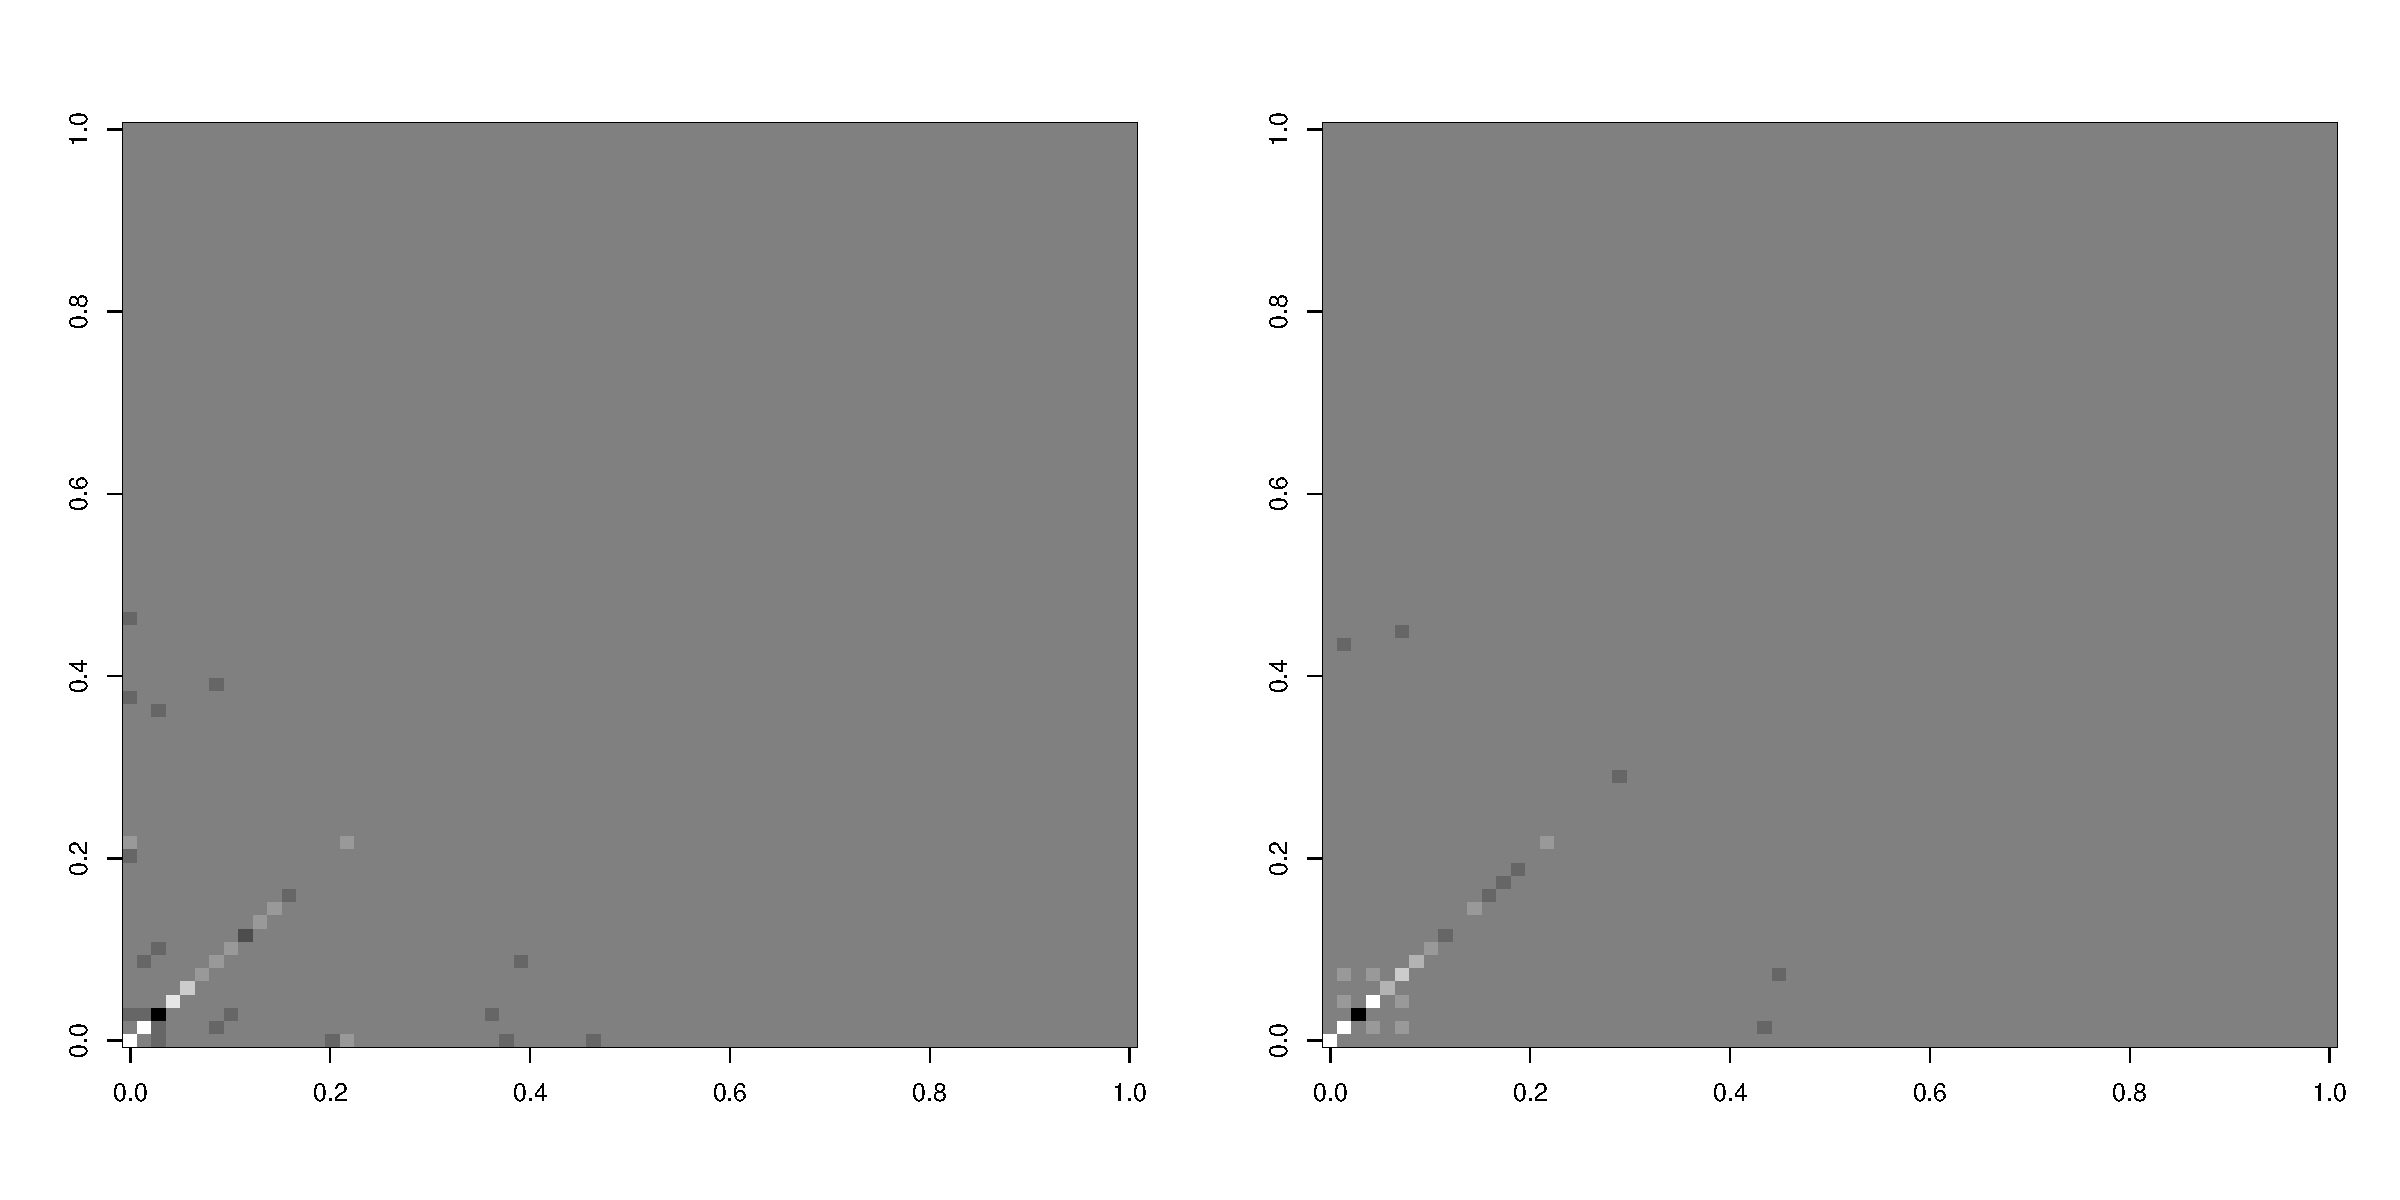
\includegraphics[width=1\textwidth]{D}
\caption{Estimated $\tilde D_i$ for $2$ random subjects showing that the empirically chosen factor induces high sparsity. Gray dots are the elements with value close to $0$, while white dots are far from 0.}
\label{demoD}
\end{figure}

As an illustration, I use $m=200$ adjacency matrices, each of size $70 \times 70$ and a weakly informative prior $\tau_{i,jk}=1000$ for all $\tilde D_{i,jk}$. In order to demonstrate that the empirical factor induces a low-rank and near-diagonal core, I set the core to be full rank and this prior to temporarily not enforcing any structure (e.g. sparsity, low rank, etc) as a-priori. The posterior of $\tilde D_i$ is plotted in Figure~\ref{demoD}. High sparsity can be observed and each $D_i$ seems to be very close to a low-rank diagonal matrix.

\subsection{Shrinkage on the Scale of $D_i$}

Setting each factor to be square requires a full-rank parameterization of $\tilde D_{i,jk}$, but due to the sparsity, it can be significantly simplified. Therefore, I assign a shrinkage prior on $\tau_{i,jk}$ to effectively reduce most of parameters in $\tilde D_{i,jk}$ to be close to $0$.

\be
\tau_{i,jk}= \lambda^{(1)}_j \lambda^{(1)}_k \gamma_{jk}\tau_0 \quad i=1,\ldots,m,\\
\gamma_{j,k} \sim g, \quad \tau_0 \sim f,\\
(\lambda^{(1)}_1,\ldots, \lambda^{(1)}_n) \sim \text{Dirichlet} (\alpha_1, \ldots \alpha_1)
\ee

Since the aim of this application is to obtain an equal-dimension low dimensional array for each subject, I let $\tau_{i,jk}$ to be the same for all $i$; the product of $\lambda^{(1)}_j \lambda^{(1)}_k$ ensures the shrinkage is applied symmetrically in each $\tilde D_i$; $g$ is a heavy-tail distribution such as Laplace to allow large signal. When the tensor is of higher order $p$ and non-symmetric, the following can be used:

\be
\tau_{i,j_1\ldots j_p}= \lambda^{(1)}_{j_1} \lambda^{(2)}_{j_2}, \ldots \lambda^{(p)}_{j_p}\gamma_{j_1\ldots j_p} \tau_0\\
\gamma_{j_1\ldots j_p} \sim g, \quad \tau_0 \sim f,\\
(\lambda^{(1)}_1,\ldots, \lambda^{(1)}_{n_1}) \sim \text{Dirichlet} (\alpha_1, \ldots \alpha_1)\\
\vdots\\
(\lambda^{(p)}_1,\ldots, \lambda^{(p)}_{n_p}) \sim \text{Dirichlet} (\alpha_p, \ldots \alpha_p)
\ee

% \subsection{Issues to address?}

% There are a couple of issues:

% 1. Computing burden on global-local shrinkage:

% Let the rank of the core tensor be equal to the original tensor theoretically justifies the use of the empirical factor. But with a global-local shrinkage, sampling the local scale $\gamma_{j_1\ldots j_p}$ would be horrendous. Maybe there is a more efficient parameterization?

% 2. Alternative core structure:

% Another idea to describe the core structure, instead of using shrinkage via scale prior. Directly model the core as another PARAFAC decomposition and apply the multiway shrinkage to induce a sparse core? We might get away with the non-identifiability issue of PARAFAC since we only care about the tensor estimate of the core.



\end{document}
